\documentclass[a4paper]{article}
\usepackage{geometry}
\usepackage[utf8]{inputenc}
\usepackage{amsmath}
\usepackage{graphicx}
\usepackage{subcaption}
\usepackage{hyperref}

\graphicspath{{./figs/}}

\newcommand{\nfit}{ \texttt{n3fit} }
\newcommand{\dcs}{ \Delta_{\chi^{2}} }
\newcommand{\vphys}{ \texttt{validphys} }
\newcommand{\chis}{ \chi^{2} }
\newcommand{\thc}{\langle T \rangle}
\newcommand{\T}[1]{{#1}^{\mathrm{T}}}

\title{Closure Test studies with n3fit}
\author{Michael Wilson}
\date{April 2019}

\begin{document}

\maketitle

\section{Introduction}

We have seen that the new \nfit code gives us access to very powerful and
modern fitting tools. With great power comes great responsibility, we have already
seen examples of some kind of overfitting with the new code - producing PDFs
with wiggly behaviour and incredibly good fits to the data. This affect is
well demonstrated in the \nfit paper and can be seen in Figure \ref{fig:v3pdf}

\begin{figure}[!h]
    \centering
    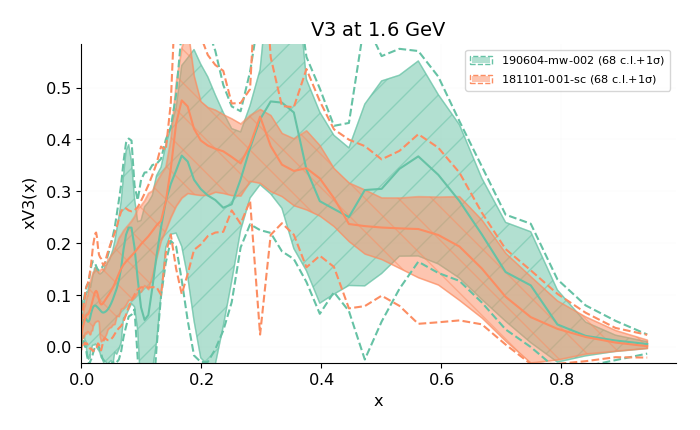
\includegraphics[width=0.8\textwidth]{plot_pdfs_V3.png}
    \caption{
        Figure showing wiggly behaviour of v3 PDF when using the new fitting code.
        }
    \label{fig:v3pdf}
\end{figure}

This leaves us with a few questions: Can we discriminate against this
architecture/minimiser choice in a closure test using the closure estimators?
Is this just flat directions in the DIS only fit? Is there a good prescription
for combatting this effect.

There has already been a study purely on the data which shows that by having a test
set which is used in the hyper parameter scan which seperates out completely a dataset
or series of datasets the hyper optimiser lands on a notably smaller network which reduces
the amount of redundant features in the PDF. Do we need to consider the same kind of test
set in the closure tests so that the closure test estimators can be calculated both in and
out of sample - where in sample refers to the dataset appearing in either the training
or validation set which is used for stopping.

\section{re-examining closure test estimators}

Previously we motivated two additonal closure test estimators, in the space of data
which in addition to the pre-existing $\dcs$ makes 3 estimators which are currently
included in the \vphys closure report. To recap those estimators are:

\subsection*{Bias}

The bias is defined as the $\chis$ between the central theory prediction, $\thc$,
and the level 0 data, $D_{0}$. This is clearly a measure of how far away the
central prediciction is away from the underlying law, explictly defined as

\begin{equation}
    \mathrm{bias} = \frac{1}{N_{\mathrm{data}}} \T{(\thc - D_{0})} C^{-1} (\thc - D_{0})
\end{equation}

where we have normalised over the number of data points $N_{\mathrm{data}}$. Ideally this should
be minimised, but this isn't always so simple - adding parameters to the model
typically lowers the bias as the model has freedom to fit the data better, however at some point the
cost for lowering the bias is that the variance of the model increases, which brings us to the second
statistical estimator

\subsection*{Variance}

This quantity goes alongside the bias and tells us the variability of the $\chis$ with the model. We
already use this estimator in the fits, by a different name $\varphi$, in the case of a closure
defined as

\begin{equation}
    \begin{split}
        \mathrm{variance} &= \frac{1}{N_{\mathrm{rep}} N_{\mathrm{data}}} \sum_{k} \T{(\thc - T_{k})} C^{-1} (\thc - T_{k}) \\
        &= \frac{1}{N_{\mathrm{rep}}} \left[ \langle \chis \left[ T_{k}, D_{1} \right] \rangle - \chis[\thc, D_{1}] \right]
    \end{split}
\end{equation}

where $\langle \cdot \rangle$ should be understood as the mean across replicas. We see
that the variance is just the average spread of replicas in the space of $\chis$.
Generally the aim of fitting is to reduce the bias whilst retaining a reasonable
variance - this is commonly referred to as the bias-variance tradeoff.

\subsection*{Delta chi2}

We now turn to the final estimator - $\dcs$. The estimator was introduced in the
3.0 paper alongside the closure test and was described as an estimator which told
us how well the fit reproduced the underlying law. Here we will refine this definition
with the help of the bias.

We start with the definition of the $\dcs$

\begin{equation}
    \dcs = \frac{\chis[\thc, D_{1}] - \chis[D_{0}, D_{1}]}{\chis[D_{0}, D_{1}]}
\end{equation}
the notation here differs slightly from the original notatation, but we can understand
the $D_{0}$ as the theory prediction of the central input PDF. There were bounds given alongside
$\dcs$ which described when the fit was overfitting

\begin{itemize}
    \item $\dcs < 0$ overfitting
    \item $\dcs = 0$ perfect fit
    \item $\dcs > 0$ underfitting 
\end{itemize}

although these bounds intuitively make sense, it's not entirely clear if these
bounds have any connection to the bias. If the bias increases but the $\dcs$ becomes
less negative, do we understand this is a better or worse fit, and is that even consistent
with the definition of overfitting given above?

We can rephrase $\dcs$ in terms of the bias to help us here:

\begin{equation}
    \begin{split}
        \dcs &= \frac{\chis[\thc, D_{1}] - \chis[D_{0}, D_{1}]}{\chis[D_{0}, D_{1}]} \\
        &= \frac{\chis[\T{(\thc - D_{1})} C^{-1} (\thc - D_{1}) - \chis[D_{0}, D_{1}]}{\chis[D_{0}, D_{1}]} \\
        &= \frac{\chis[\T{(\thc - D_{0} + D_{0} - D_{1})} C^{-1} (\thc - D_{0} + D_{0} -D_{1}) - \chis[D_{0}, D_{1}]}{\chis[D_{0}, D_{1}]} \\
        &= \frac{ \chis[\thc, D_{0}] + 2 \T{(\thc - D_{0})} C^{-1} (D_{0} - D_{1}) }{\chis[D_{0}, D_{1}]}
    \end{split}
    \label{eq: deltachi2tobias}
\end{equation}

we recognise the first term in the numerator as the bias, the second term is not
instantly recognisable. However we know the shift, $D_{0} - D_{1}$ by construction

\begin{equation}
    \begin{split}
        D_{0} - D_{1} &\equiv - \eta \\
        &= - \sum_{i} \sigma_{i} \epsilon_{i} v_{i}
    \end{split}
\end{equation}

where $\epsilon$ is a normally distributed number, $\sigma_{i}$ is the square root
of the $i^{\mathrm{th}}$ eigenvalue of the covariance matrix and $v_{i}$ is the
corresponding eigenvector. We can leverage this to simplify the last line of
\eqref{eq: deltachi2tobias}.

\begin{equation}
    \dcs = \frac{ \chis[\thc, D_{0}] - 2 \sum_{i} \T{(\thc - D_{0})} \sigma_{i}^{-1} \epsilon_{i} v_{i} }{ \sum_{i} \epsilon_{i}^{2} }
\end{equation}

if we move to the basis that diagonalises the covariance matrix this can be simplified to

\begin{equation}
    \dcs = \frac{ \sum_{i}^{N_{\mathrm{data}}} \big[ 
        \frac{(\hat{\thc} - \hat{D_{0}})_{i} (\hat{\thc} - \hat{D_{0}})_{i}}{\sigma_{i}^{2}} -
        2 \frac{(\hat{\thc} - \hat{D_{0}})_{i} \hat{\eta}_{i}}{\sigma_{i}^{2}} \big] }{
            \sum_{i}^{N_{\mathrm{data}}} \epsilon_{i}^{2} }
\end{equation}

where we have used the notation that $\hat{\cdot}$ implies a vector in the
diagonal basis. The denominator is simply a normalisation constant, and in the
limit of infinite data tends to $N_{\mathrm{data}}$. The numerator can be understood
as the pull of the central prediction on the level 0 data squared (bias)
minus two times the pull of the central prediction on the level 0 times the pull
of the level 1 data on the level 0 data. We now see that $\dcs < 0$ corresponds
to the theory prediction moving away from the level 0 data specifically in the
direction of the level 1 data. $\dcs = 0$ does not necessarily refer to a perfect
fit but rather that the theory prediction is somewhere between the level 1 shift
and the underlying law such that the numerator cancels. Finally $\dcs > 0$ refers
to the theory prediction moving away from the underlying law but not towards the
level 1 data, which suggests a poor fit. 

These new definitions are not in conflict with the original bounds above but
offer a bit more insight into the subtle cases where both the bias can increase,
but $\dcs$ becomes closer to zero.

We can visualise the above with simple diagrams

\begin{figure}[!h]
    \centering
    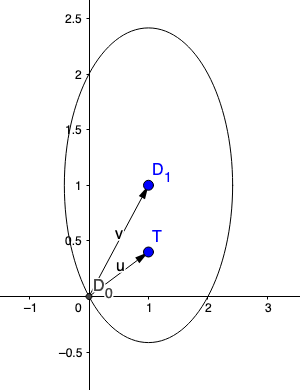
\includegraphics[width=0.4\textwidth]{vectorexample2.png}
    \caption{example in 2D to visualise $\dcs$ in the diagonal basis, the axis
    is in units of $\sigma_{i}$. $\dcs$ can be understood as the pull of
    $\thc$ squared minus two times the dot product of pull of $\thc$ and pull of
    level 1 data. $\dcs = 0$ for the given level 1 shift (in this case
    $\epsilon_1, \epsilon_2 = 1$) is fulfilled at any point on the ellipsoid and
    $\dcs<0$ and $\dcs>0$ refer to the regions inside and outside the ellipsoid
    respectively.}
    \label{fig:vectorexample}
\end{figure}

It's clear that the full story of whether a fit is better or not is given not
by a single estimator, but rather on the 3 estimators combined. We now turn to
some example results from level 2 closure tests with the \nfit code to see if we
can say something about the different architectures used in each one.

\section{results}

\subsection{Closure on pseudodata from large architecture PDF}

As a sanity check we can run a closure test with the higher parameterisation
which gave wiggly PDFs in a fit to pseudo data which is generated from the
wiggly PDF. This is to see if the features we see in the space of the PDF are
somehow picked up by the data in such a way that we can refit the same underlying
function.

This is a brute force way of trying to understand whether the features in the PDF
are just flat directions in the loss or are some kind of feature of the data. To
test this I am taking as input a wiggly PDF, and then just generating the MC
replica (level 2) noise on top of this, and so there is no level 1 fluctuation.
The test is to see if the functional form of the replicas matches the input PDF.

The full report comparing the closure fit to underlying can be found here:
\href{https://vp.nnpdf.science/tHdjyBVTQEOlfkNjUXPMFQ==}{\bf{report}}

The closure tests estimators are not particularly useful here, largely because
there is no level 1 noise. The main feature is the PDF plots are much smoother
for the closure in nearly all instances, which suggests that the extra features
in the underlying PDF are not translated into the space of data by the
\texttt{FastKernel} tables.

From this test we are would be persuaded that the underlying PDF was just fitting
flat directions in the loss and that the fluctuations in the PDF shouldn't be
taken too seriously.

\subsection{Closures with different level 1 shift}

A second sanity check was to run two different closures changing nothing but the
seed used to generate the level 1 shifts on the pseudodata. This was a test I
wanted to run to check how important it was that we considered two closures ran
not only on the same datasets but also with the same level 1 noise. In other
words, how robust are the statistical estimators on the level 1 noise? In particular
we added bootstrap sampling to some of the statistical estimators and it would
be good to know if the errorbar given by a bootstrap represents the distribution
under different level 1 shifts.

The full report can be found here:
\href{https://vp.nnpdf.science/mbcTUd6-TQmQFvaGd37bkg==}{\bf{report}}. In particular
one will note that the variance is unchanged within statistics as you would expect
but the bias and the $\dcs$ both appear to depend heavily on the level 1 noise.

This serves as a warning that the closure tests should be ran with the same level
1 data if they are to be compared.


\subsection{Closures on \texttt{MSTW2008nlo68cl}}

Now we take the smooth \texttt{MSTW2008nlo68cl} as input. We fit this
with both the conservative architecture, roughly corresponding to the number of
parameters used in NNPDF3.1, and the larger architecture found by the hyperopt
routine. The objective here is to see if we can use the closure test estimators
to distinguish and discriminate between the two fits.

All reports can be found on Wiki

Report to underlying for conservative architecture:
\href{https://vp.nnpdf.science/9qr4qCK2RHePHehBpgxBdQ==/}{\bf{report}}

larger architecture:
\href{https://vp.nnpdf.science/pdm9Y1fjTw21nhlzjzErjw==/}{\bf{report}}

Comparison report:
\href{https://vp.nnpdf.science/lQjtB-lnRy263IhAYCTw1Q==/}{\bf{report}}

we see that the delta chi2 is comparable for both fits, however the bias is
is generally lower for the conservative architecture, as well as the variance.
It seems that there is a wider spread of replicas for the larger architecture,
but this hasn't improved the fit of the central replica on the underlying law.
From the value of $\dcs$ we would say, however, that the fit hasn't moved away
from the underlying law towards the level 1 data, and appears to have just
produced a worse quality fit. The lower variance is expected for the smaller
architecture, but the interesting thing is that there hasn't been a gain in
the bias.

\end{document}
